\chapter{Console I/O}
IO stands for input/output. C provides only mechanism to interact through
console using its standard library. C does not provide ways to have GUI
although that is possible with various GUI libraries most notable being
GTK. However, discussing about GTK is out of scope of this book. In this
chapter we will focus on console output facilities of C because any program we
write at this stage will be meaningless if it has no input/output. Typically
when we interact with a C program we give input using keyboard which is also
referred as \texttt{stdin} stream. The output is monitor or \texttt{stdout}
stream. There is one more stream \texttt{stderr} which is generally redirected
to monitor or a log file. For historical reasons these are known as
\texttt{FILE} stream which represents the datatype of these
streams. \texttt{FILE} is capable of representing other streams which are disk
based for example a file on your hard drive. There are more type of input
devices on a modern computer. For example, network i/o is there. Whenever you
browse web or download a file through your Internet connection network i/o comes
into play. There is an opengroup
which specifies functions for network related functions. Operating systems
like GNU/Linux are POSIX compatible which defines how network i/o will be
used. Even a printer is a special output device, a camera input, speakers
output, microphone input and so on. In this books we are concerned with
keyboard input, output on monitor and i/o using files. Other types of i/os are
out of scope of this book.

However, before we go on with i/o I would
like to present C's memory model which will be needed by our discussion of i/o
related functions. However, if things do not make sense even then please go
through it and come later to understand more. 

\section{C's Memory Model}
As you may be knowing RAM(random access memory) is the area which is used as
primary memory. Whenever we execute a program the first thing which happens is
that it gets loaded into memory. Now a binary program becomes a process when it
is running i.e. a running program is referred as process. All processes have
memory area divided into different portions. These portions are known as data
segment, stack and code or text segment. Data segment is further split in
three parts; initialized data segment, uninitialized data segment or BSS which
is name after an ancient assembler Block Started by Symbol and
heap. Initialized data segment contains initialized global variables and static
variables. For uninitialized data segment it is same as above just that the
variables are not initialized explicitly but implicitly to zero.

Heap is the largest area of memory used for dynamic memory allocation. As
you will see later that you can manage heap using \texttt{malloc(), calloc(),
realloc(),} and \texttt{free()}. Note that operating system does not manage memory
allocated for you on heap. You, the programmer, are responsible for allocating and
freeing up memory in area. If heap gets full os will use virtual memory or swap
space on hard disk. Objects allocated on heap persist across function
calls. However, there are some very nasty problems, which, come in picture when
you use heap. There are several of them. You may forget to allocate memory and
may dereference unallocated pointer. You may have initialized it to
\texttt{NULL} and try to dereference that. You may allocate and free twice. You
forgot to set pointer to \texttt{NULL} after freeing it. And last but not the
least you loose all pointers to the memory area before you can free. The nature
with this particular problem is that if your program is going to run for long
time then it is going to consume more and more memory. Because of its nature it
is known as memory leak. It is very difficult to detect such problems in code
which does not run for long periods of time. Our friend Valgrind will come to
help up with this problem. When a memory leak happens it eats up RAM slowly and
then operating system has to use virtual memory as explained above. In a
nutshell, I will say that heap means you have to manage it.

\begin{figure}[t!]
\begin{center}
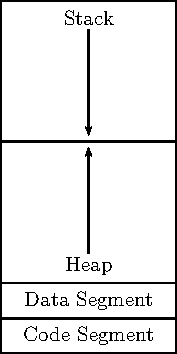
\includegraphics{figs/mem_model.pdf}
\end{center}
\caption{Memory model of a C program}
\end{figure}

Stack is relatively simple. All non-static and non-register variables go on
stack if not allocated dynamically. Stack variables do not retain there value
across function calls unless
they are passed as pointers. Also, when they go out of
scope, that is the scope in which they were declared ends, they will be kind of
lost. The way in which stack frame moves the same area will be used for new
variables. However, stack is very limited (compared to heap) and in deeply
nested function calls or recursion (you will see these in Functions chapter)
stack may get full and program may crash. The reason for crashing is that
operating system will not use virtual memory but will do a segmentation fault
in its place. GNU/Linux allow its users to modify the stack size by 
\texttt{ulimit} command. Note that stack and heap are adjacent in memory and 
grow in opposite direction.

Code segment or text segment is an area where the executable instructions of
program reside. It is typically constant and read-only area unless your system
allows self-modifying code. Following diagram shows the memory layout.

Note that this memory model not only applies to C but any process.

Now we will look at those functions, which, allow us to do console i/o. We will
begin with our familiar friends; printf and scanf.

\section{printf}
The prototype of \texttt{printf} is given by

\begin{minted}[frame=single]{c}
int printf(const char* fmt, ...);
\end{minted}

Let us take a minute to understand this as we have not yet covered
functions. The first word is \texttt{int} which denotes the return type of the
\texttt{printf} function. This is no. of characters printed. Then we have name
of the function. \texttt{fmt} is the format string of type \texttt{const
 char}. In C, strings are either character arrays or character pointers. Here,
const means \texttt{printf} will not modify the format string. The ... means
variable no. of arguments, which, can be 0 also to be supplied to
\texttt{printf}.

\texttt{printf} is a string based output function that is It writes character
strings to \texttt{stdout}. The data which has to be written is formatted by
format string as shown previously. After the format specifier it expects as
many arguments as specified in format string. The characters which are not
like, say \texttt{\%d} for example, arecalled ordinary characters. These are
simply copied to output stream, which, is stdout for printf. The \texttt{\%d}
like conversion characters are known as conversion specification or format
specifiers. Each conversion specification should be augmented with one one
argument. The results are undefined if there are insufficient arguments for the
format. If extra arguments are given the excess arguments will be evaluated but
are otherwise ignored. However, there is a big problem here! There is no
type-safety. In general compiler will warn you about it and you, the
programmer, are responsible for giving correct format string, correct no. of
correct type of arguments. Consider the following program for example:

\begin{minted}[frame=single]{c}
#include <stdio.h>

int main()
{
  printf("%d %d\n", 3, 8);

  //do not mess it. undefined behavior
  printf("%d %d\n", 5);

  //extra arguments ignored
  printf("%d %d\n", 3, 5, "hello");

  //legal because char is integer type
  printf("%d\n", 's');

  //wrap around of integer as char
  printf("%c\n", 836);

  //do not mess with type-safety
  int i = printf("%d\n", "hello");
  prinf("%d\n", i);

  return 0;
}
\end{minted}

now that if you give the command like \texttt{gcc -Wall printf.c} where
\texttt{printf.c} is the name of the file then you will be shown following
warnings:

\begin{Verbatim}[frame=single]
printf.c: In function 'main':
printf.c:8:3: warning: format '%d' expects a matching 'int' argument [-Wformat=]
   printf("%d %d\n", 5);
   ^
printf.c:8:3: warning: format '%d' expects a matching 'int' argument [-Wformat=]
printf.c:11:3: warning: too many arguments for format [-Wformat-extra-args]
   printf("%d %d\n", 3, 5, "hello");
   ^
printf.c:11:3: warning: too many arguments for format [-Wformat-extra-args]
printf.c:20:3: warning: format '%d' expects argument of type 'int', but
argument 2 has type 'char *' [-Wformat=]
   int i = printf("%d\n", "hello");
   ^
printf.c:20:3: warning: format '%d' expects argument of type 'int', but
argument 2 has type 'char *' [-Wformat=]
\end{Verbatim}

Clearly this is not a good sign for any program. A program should compile
cleanly. In our case \texttt{gcc} is generating binary even though there are
warnings. You can make \texttt{gcc} generate more warnings by issuing a
\texttt{-Wall} flag. You can also treat all warnings as errors by passing
\texttt{-Werror} to \texttt{gcc}. These two options will ensure that your code
has no warnings. Now let us move to output and try to understand it. The output
on my system is as given below. It may differ on your system:
\\\\\texttt{3 8\\
5 8\\
3 5\\
115\\
D\\
134514119\\
10\\\\}
First \texttt{printf} is correct as expected. The second line causes undefined
behavior. You may think it is the previous 8 but believe me it is not
guaranteed that it will always the case. Ii is \textbf{UNDEFINED}. Third
\texttt{printf} is also fine in the sense that extra argument is
ignored. Fourth and fifth are normal. Sixth is again a big problem. You are
trying to print a decimal integer while argument is a character string. There
is no way for compiler to determine that what should be printed which will fit
on standards.

A full detail of all conversion specification is given in specification at \S(iso.7.21.6).

In real-world most of the time the conversion specifiers are kept simple. Given
below is a sample program showing some of the things given above:

\begin{minted}[frame=single]{c}
#include<stdio.h>

int main()
{
  int i   = 343456;
  float f = 123;
  long double ld = 78939.9347;

  printf("% d\n", i);
  printf("%+d\n", i);
  printf("%#o\n", i);
  printf("%#f\n", f);
  printf("%-08i\n", i);
  printf("%08i\n", i);
  printf("%8i\n", i);
  printf("%hhi\n", i);
  printf("%hi\n", i);
  printf("%li\n", i);
  printf("%lli\n", i);
  printf("%ji\n", i);
  printf("%zi\n", i);
  printf("%ti\n", i);
  printf("%8.8f\n", f);
  printf("%8.8Lf\n", ld);

  return 0;
}
\end{minted}

The output of the above program is:
\\\\\texttt{ 343456\\
+343456\\
01236640\\
123.000000\\
343456\\
00343456\\
  343456\\
-96\\
15776\\
343456\\
4638355772471066016\\
4638355772471066016\\
343456\\
343456\\
123.00000000\\
78939.93470000\\\\}
We will keep seeing more conversion specifiers being used as we progress
through this book.

\section{scanf}
The prototype of \texttt{scanf} is given below which is very similar to
\texttt{printf}.

\begin{minted}[frame=single]{c}
int scanf(const char * restrict format, ...);
\end{minted}
It scans \texttt{stdin} or keyboard for input. Its signature is same as that of
\texttt{printf()}. It reads bytes from keyboard input, interprets them
according to format string. It also expects a set of pointer arguments as
opposed to values for printf(). The pointers indicate where the interpreted
data from the input will be stored. The result is \texttt{UNDEFINED} if there
are less number of pointer arguments than the number of conversion specifiers in
format string. Excess arguments will be evaluated but ignored. The format
string can have only white-space characters or an ordinary character (neither
`\%' nor a white-space character) or a conversion specification. Each
conversion specification is introduced by `\%', after which the following
appear in sequence.

For now if you do not understand what is a pointer then let us have a simple
definition for that. A pointer is a variable which stores a memory location
where the value will be stored.

The full detail of conversion specification can be found at \S(iso.7.12.6.2)
which lists \texttt{fscanf} function but conversion specifiers are same for
both.

Now that we have seen this description let us take a look at few examples.

\begin{minted}[frame=single]{c}
#include <stdio.h>

int main()
{
  char str[128] = {0};

  scanf("%s", str);
  printf("You entered:\n%s\n", str);

  return 0;
}
\end{minted}

and the output is:
\\\\\texttt{\textbf{Hi! My name is Shiv.\\}
You entered:\\
Hi!\\\\}
It is certainly not the correct output. We had expected to see like: ``Hi! My
name is Shiv.''. What happened to input string after ``Hi!''. Well, in a form
given above for \texttt{scanf()} it will stop taking input after white-space
for character strings. For numerics it does not matter as it does not match the
format. For characters it is character-by-character so no confusion either. So
what if you want to have the entire string including white-spaces. Use
\texttt{[\^{}n]} as given below:

\begin{minted}[frame=single]{c}
#include <stdio.h>

int main()
{
  char str[128] = {0};

  scanf("%[^\n]s", str);
  printf("You entered:\n%s\n", str);

  return 0;
}
\end{minted}

and the output is:
\\\\\texttt{\textbf{Hi! My name is Shiv.}\\
You entered:\\
Hi! My name is Shiv.\\\\}
What if you want to filter a string based on certain patterns. For example, a
character string does not contain more that a single space, English alphabets,
period and digits. To scan such a string you can define a pattern as program
given below shows:

\begin{minted}[frame=single]{c}
#include <stdio.h>

int main()
{
  char c[100]={0};

  scanf("%[ A-Za-z0-9!.]", c);
  printf("%s\n", c);

  return 0;
}
\end{minted}

and the output is:
\\\\\texttt{\textbf{Hi! My name is Shiv! My phone no. is 1234. \%\^\$\&\*\\}
Hi! My name is Shiv! My phone no. is 1234.\\\\}
There is also a major problem associated with input and that comes when you
have characters involved. Consider the following program:

\begin{minted}[frame=single]{c}
#include <stdio.h>

int main()
{
  int   i = 0;
  float f = 0.0;
  char  c1 = '\0';
  char  c2 = '\0';
  char  c3 = '\0';

  printf("Enter an integer, a float and three character one by one:\n");

  scanf("%d", &i);
  scanf("%f", &f);
  scanf("%c", &c1);
  scanf("%c", &c2);
  scanf("%c", &c3);

  printf("You entered\n");
  printf("%d\n", i);
  printf("%f\n", f);
  printf("%c\n", c1);
  printf("%c\n", c2);
  printf("%c\n", c3);

  return 0;
}
\end{minted}

and the output is:
\\\\\texttt{\textbf{2\\
3.4\\
s\\}
You entered\\
2\\
3.400000\\
\\
\\
s\\\\}
What is happening here is that newline entered by our RET key is getting
assigned to \texttt{c1} and \texttt{c3}. That is why the program accepted only
second character. The enter after \texttt{float f;} was assigned to \texttt{c1}
and the character entered to \texttt{c2} and then the RET newline to
\texttt{c3}. There is a very simple way to recover from this:

\begin{minted}[frame=single]{c}
#include <stdio.h>

int main()
{
  int   i = 0;
  float f = 0.0;
  char  c1 = '\0';
  char  c2 = '\0';
  char  c3 = '\0';

  printf("Enter an integer, a float and three character one by one:\n");
  scanf("%d", &i);
  scanf("%f", &f);
  scanf(" %c", &c1);
  scanf(" %c", &c2);
  scanf(" %c", &c3);

  printf("%d\n", i);
  printf("%f\n", f);
  printf("%c\n", c1);
  printf("%c\n", c2);
  printf("%c\n", c3);

  return 0;
}
\end{minted}

The whitespace character shown will eat up all the white-space given after the
previous input. This concludes our discussion on \texttt{printf()} and
\texttt{scanf()}. Now we will move to another set of i/o functions which take
character string without filtering and print it to screen without
filtering. What I am going to discuss are \texttt{gets(), fgets(), puts()} and
\texttt{fputs()}.

All the following function's reference is present in \S(iso.7.21) which deals with
header `stdio.h`.

\section{Sting I/O Functions}
These functions are very simple compared to \texttt{printf(}) and
\texttt{scanf()}. They take a pointer to a character array or a character
pointer and fill it with input or print it to monitor. Note that
\texttt{gets()} and \texttt{puts()} work only with \texttt{stdin} and
\texttt{stdout} respectively while \texttt{fgets()} and \texttt{fputs()} work
with \texttt{FILE} streams i.e. other than \texttt{stdin} and \texttt{stdout}
they can also work with disk based files. Here is a sample program:

\begin{minted}[frame=single]{c}
#include <stdio.h>
#include <stdlib.h>

int main()
{
  char cStack[1024] = "";
  char *cHeap = (char*)malloc(sizeof(1024));

  gets(cStack);
  puts(cStack);

  cHeap = fgets(cHeap, 1024, stdin);
  fputs(cHeap, stdout);

  return 0;
}
\end{minted}

and the output is:
\\\\\texttt{\textbf{Hi!\\}
Hi!\\
\textbf{Hello!\\}
Hello!\\\\}
First \texttt{``Hi!''} and \texttt{``Hello!''} are keyboard inputs. Do not
worry about array and pointer syntax at the moment. Just see the difference
between function calls. Their is a problem with \texttt{gets()} that it can
cause buffer overflow. If input is bigger than 1024 bytes including the null
terminator then buffer overflow will happen. Note how you can prevent it with
\texttt{fgets()} by specifying the number of characters you want to read. Rest
of input will be ignored by \texttt{fgets()}. This is a security hole and
therefore you should never ever use \texttt{gets()}.

\section{Character I/O Functions}
There are several functions for single character i/o. They are \texttt{getc(),
  putc(), getchar(), putchar(), fgetc()} and \texttt{fputc()}. Apart from
\texttt{getchar()} and \texttt{putchar()} rest can do any FILE stream-based
i/o. Let us have a simple program as they are mostly trivial.

\begin{minted}[frame=single]{c}
#include<stdio.h>

int main()
{
  char c ='';

  c = getchar();
  putchar(c);

  c = getchar();
  putchar(c);

  c = fgetc(stdin);
  fputc(c, stdout);

  c = getchar();
  putchar(c);

  c = getc(stdin);
  putc(c, stdout);

  return 0;
}
\end{minted}

and the output is:
\\\\\texttt{\textbf{4\\}
4\\
\textbf{5\\}
5\\
\textbf{6\\}
6\\\\}
The first 4, 5 and 6 were keyboard inputs. Note the use of extra
\texttt{getchar()} and \texttt{putchar()} to handle the situation we faced
during \texttt{scanf()}.


